\documentclass[11pt]{article}

\usepackage[margin=1in]{geometry}
\usepackage{amsmath}
\usepackage{amssymb}
\usepackage{graphicx}

\title{705.641.81: Homework 1}
\author{David Carrillo}
\date{}

\begin{document}
\maketitle

\section{Linear Algebra Review}
\subsection{Basic Operations}

With $\alpha = 2$, $\mathbf{x} = [0,1,2]^\top$, $\mathbf{y} = [3,4,5]^\top$,
$\mathbf{z} = [1,2,-1]^\top$, and
$A = \begin{bmatrix} 3&2&2\\1&3&1\\1&1&3\end{bmatrix}$:

\begin{enumerate}
  \item $\sum_{i=1}^{n} x_i y_i = (0)(3) + (1)(4) + (2)(5) = 0 + 4 + 10 = \mathbf{14}$.

  \item $\sum_{i=1}^{n} x_i z_i = (0)(1) + (1)(2) + (2)(-1) = 0 + 2 - 2 = \mathbf{0}$.
        The inner product vanishes, which is what makes $\mathbf{x}$ and $\mathbf{z}$ orthogonal.

  \item $\alpha(\mathbf{x} + \mathbf{y}) = 2[0+3,\ 1+4,\ 2+5]^\top = 2[3,5,7]^\top = [6,10,14]^\top$.

  \item $\|\mathbf{x}\| = \sqrt{0^2 + 1^2 + 2^2} = \sqrt{5} \approx \mathbf{2.2361}$.

  \item $\mathbf{x}^\top = \begin{bmatrix} 0 & 1 & 2\end{bmatrix}$, the $1 \times 3$ row vector
        obtained from the $3 \times 1$ column $\mathbf{x}$.

  \item $A\mathbf{x}$: each entry is a row of $A$ dotted with $\mathbf{x}$,
        \[
          A\mathbf{x} =
          \begin{bmatrix}
            (3)(0) + (2)(1) + (2)(2)\\
            (1)(0) + (3)(1) + (1)(2)\\
            (1)(0) + (1)(1) + (3)(2)
          \end{bmatrix}
          =
          \begin{bmatrix} 6 \\ 5 \\ 7 \end{bmatrix}.
        \]

  \item $\mathbf{x}^\top A \mathbf{x} = \mathbf{x} \cdot (A\mathbf{x})
        = (0)(6) + (1)(5) + (2)(7) = 0 + 5 + 14 = \mathbf{19}$.
\end{enumerate}

\subsection{Matrix Algebra Rules}

Here $\{\mathbf{x},\mathbf{y},\mathbf{z}\}$ are $n \times 1$ column vectors and $\{A,B,C\}$ are
$n \times n$ real matrices.

\begin{enumerate}
  \item $\mathbf{x}^\top\mathbf{y} = \sum_{i=1}^{n} x_i y_i$. \textbf{True.} This is the definition of the
        inner product: the $(1\times n)(n \times 1)$ product is the $1 \times 1$ sum of elementwise products.

  \item $\mathbf{x}^\top\mathbf{x} = \|\mathbf{x}\|^2$. \textbf{True.} Setting $\mathbf{y} = \mathbf{x}$
        above gives $\sum_i x_i^2$, which is the definition of the squared Euclidean norm.

  \item $\mathbf{x}^\top\mathbf{x} = \mathbf{x}\mathbf{x}^\top$. \textbf{False.} The shapes do not even
        match: $\mathbf{x}^\top\mathbf{x}$ is $1 \times 1$ while $\mathbf{x}\mathbf{x}^\top$ is
        $n \times n$. For $\mathbf{x} = [1,2,3]^\top$, $\mathbf{x}^\top\mathbf{x} = 14$ but
        $\mathbf{x}\mathbf{x}^\top = \begin{bmatrix} 1&2&3\\2&4&6\\3&6&9\end{bmatrix}$, a rank-one matrix.

  \item $(\mathbf{x}-\mathbf{y})^\top(\mathbf{y}-\mathbf{x}) = \|\mathbf{x}\|^2 -
        2\mathbf{x}^\top\mathbf{y} + \|\mathbf{y}\|^2$.
        \textbf{False}, and the error is a sign. Since $\mathbf{y}-\mathbf{x} = -(\mathbf{x}-\mathbf{y})$,
        \[
          (\mathbf{x}-\mathbf{y})^\top(\mathbf{y}-\mathbf{x})
          = -(\mathbf{x}-\mathbf{y})^\top(\mathbf{x}-\mathbf{y})
          = -\|\mathbf{x}-\mathbf{y}\|^2
          = -(\|\mathbf{x}\|^2 - 2\mathbf{x}^\top\mathbf{y} + \|\mathbf{y}\|^2).
        \]
        The left side is $\le 0$ always, while the right side is $\ge 0$ always. They agree only when
        $\mathbf{x} = \mathbf{y}$. With $\mathbf{x} = [1,2,3]^\top$ and $\mathbf{y} = [0,1,0]^\top$ the
        left side is $-11$ and the right side is $+11$. The correct identity uses
        $(\mathbf{x}-\mathbf{y})^\top(\mathbf{x}-\mathbf{y})$.

  \item $AB = BA$. \textbf{False.} Matrix multiplication does not commute. With
        $A = \begin{bmatrix} 1&1\\0&1\end{bmatrix}$ and $B = \begin{bmatrix} 1&0\\1&1\end{bmatrix}$,
        $AB = \begin{bmatrix} 2&1\\1&1\end{bmatrix}$ but $BA = \begin{bmatrix} 1&1\\1&2\end{bmatrix}$.

  \item $A(B+C) = AB + AC$. \textbf{True.} Matrix multiplication distributes over addition, since
        $\sum_k a_{ik}(b_{kj} + c_{kj}) = \sum_k a_{ik}b_{kj} + \sum_k a_{ik}c_{kj}$.

  \item $(AB)^\top = A^\top B^\top$. \textbf{False.} The transpose reverses the order:
        $(AB)^\top = B^\top A^\top$. With the same $A$ and $B$ as above,
        $(AB)^\top = \begin{bmatrix} 2&1\\1&1\end{bmatrix}$ and
        $A^\top B^\top = \begin{bmatrix} 1&1\\1&2\end{bmatrix}$, which differ, while
        $B^\top A^\top = \begin{bmatrix} 2&1\\1&1\end{bmatrix}$ matches.

  \item $\mathbf{x}^\top A \mathbf{y} = \mathbf{y}^\top A^\top \mathbf{x}$. \textbf{True.} The quantity
        $\mathbf{x}^\top A \mathbf{y}$ is $1 \times 1$, so it equals its own transpose, and
        $(\mathbf{x}^\top A \mathbf{y})^\top = \mathbf{y}^\top A^\top \mathbf{x}$ by reversing the order
        of the three factors.

  \item $A^\top A = I$ is the columns of $A$ are orthonormal. \textbf{True.} Writing
        $A = [\mathbf{a}_1 \cdots \mathbf{a}_n]$ by columns, the $(i,j)$ entry of $A^\top A$ is
        $\mathbf{a}_i^\top\mathbf{a}_j$. So $A^\top A = I$ says exactly that
        $\mathbf{a}_i^\top\mathbf{a}_j = 0$ for $i \ne j$ and $\mathbf{a}_i^\top\mathbf{a}_i = 1$, which is
        the definition of an orthonormal set of columns. The implication runs both ways.
\end{enumerate}

\subsection{Matrix operations}

Let $B = \begin{bmatrix} 1&-1&0\\-1&2&-1\\0&-1&1\end{bmatrix}$.

\subsubsection*{Is $B$ invertible?}

No. Expanding the determinant along the first row,
\[
  \det B = 1[(2)(1) - (-1)(-1)] - (-1)[(-1)(1) - (-1)(0)] + 0 = 1(2 - 1) + 1(-1) = 1 - 1 = 0.
\]
A zero determinant means $B$ is singular, so $B^{-1}$ does not exist. The reason is visible in the
structure: every row sums to zero, so $B[1,1,1]^\top = \mathbf{0}$ and the vector $[1,1,1]^\top$ spans
the null space. The rank is 2.

\subsubsection*{Is $B$ diagonalizable?}

Yes. The characteristic polynomial is
\[
  \det(B - \lambda I) = (1-\lambda)[(2-\lambda)(1-\lambda) - 1] + 1[-(1-\lambda)]
  = (1-\lambda)[(2-\lambda)(1-\lambda) - 2],
\]
and since $(2-\lambda)(1-\lambda) - 2 = \lambda^2 - 3\lambda = \lambda(\lambda - 3)$,
\[
  \det(B - \lambda I) = (1-\lambda)\lambda(\lambda-3),
  \qquad \text{so} \qquad
  \lambda \in \{0, 1, 3\}.
\]
Three distinct eigenvalues in a $3 \times 3$ matrix give three linearly independent eigenvectors, so
$B$ is diagonalizable. It is also real symmetric, so the spectral theorem guarantees this independently.
Solving $(B - \lambda I)\mathbf{v} = \mathbf{0}$ for each eigenvalue:
\[
  \lambda_1 = 0: \ \mathbf{v}_1 = \begin{bmatrix} 1\\1\\1\end{bmatrix}, \qquad
  \lambda_2 = 1: \ \mathbf{v}_2 = \begin{bmatrix} -1\\0\\1\end{bmatrix}, \qquad
  \lambda_3 = 3: \ \mathbf{v}_3 = \begin{bmatrix} 1\\-2\\1\end{bmatrix}.
\]
The diagonalization is $B = PDP^{-1}$ with
\[
  P = \begin{bmatrix} 1&-1&1\\1&0&-2\\1&1&1\end{bmatrix}, \qquad
  D = \begin{bmatrix} 0&0&0\\0&1&0\\0&0&3\end{bmatrix}.
\]
Because $B$ is symmetric its eigenvectors are mutually orthogonal, so normalizing the columns of $P$
gives an orthogonal $Q$ with $B = QDQ^\top$:
\[
  Q = \begin{bmatrix}
    1/\sqrt{3} & -1/\sqrt{2} & 1/\sqrt{6}\\
    1/\sqrt{3} & 0 & -2/\sqrt{6}\\
    1/\sqrt{3} & 1/\sqrt{2} & 1/\sqrt{6}
  \end{bmatrix}.
\]

\section{Taking Chances: Probability Review}

\subsection{Basic probability}

\begin{enumerate}
  \item Two dice give $6 \times 6 = 36$ equally likely ordered outcomes. Counting by absolute difference
        $d = |d_1 - d_2|$, there are $12 - 2d$ outcomes for each $d \ge 1$, so $d = 3$ gives 6 outcomes,
        $d = 4$ gives 4, and $d = 5$ gives 2. The winning event $d \ge 3$ therefore has
        $6 + 4 + 2 = 12$ outcomes:
        \[
          \mathbb{P}(\text{win}) = \frac{12}{36} = \frac{1}{3}.
        \]
        The payoff is \$15 on a win and \$0 otherwise, so
        $\mathbb{E}[\text{payoff}] = 15 \cdot \frac{1}{3} + 0 \cdot \frac{2}{3} = \$5$.
        A fair ticket price is \textbf{\$5}, the price at which the game has zero expected profit.

  \item From $\mathbb{P}(A \cup B) = \mathbb{P}(A) + \mathbb{P}(B) - \mathbb{P}(A,B)$ with
        $\mathbb{P}(A,B) = 0$:
        \[
          0.95 = 0.4 + \mathbb{P}(B) - 0,
          \qquad \text{so} \qquad
          \mathbb{P}(B) = \mathbf{0.55}.
        \]

  \item If $A$ and $B$ are independent then
        $\mathbb{P}(A,B) = \mathbb{P}(A)\mathbb{P}(B) = 0.4\mathbb{P}(B)$, so
        \[
          0.95 = 0.4 + \mathbb{P}(B) - 0.4\mathbb{P}(B) = 0.4 + 0.6\mathbb{P}(B),
          \qquad \text{so} \qquad
          \mathbb{P}(B) = \frac{0.55}{0.6} = \frac{11}{12} \approx \mathbf{0.9167}.
        \]
        Independence forces a larger $\mathbb{P}(B)$ than mutual exclusivity does, because the overlap
        $\mathbb{P}(A,B)$ is now double counted in $\mathbb{P}(A) + \mathbb{P}(B)$ and has to be made
        up for.
\end{enumerate}

\subsection{Expectations and Variance}

Each of the 3 repetitions draws a coin uniformly and flips it once, so a single trial gives heads with
probability
\[
  \mathbb{P}(\text{heads}) = \frac{1}{2}(0.3) + \frac{1}{2}(0.9) = 0.6.
\]
The coin is re-drawn on every repetition, so the three trials are independent and identically distributed
Bernoulli$(0.6)$ draws and $X \sim \text{Binomial}(3, 0.6)$. This is worth stating explicitly: $X$ is
\emph{not} a mixture of a Binomial$(3,0.3)$ and a Binomial$(3,0.9)$, which is what it would be if one coin
were chosen once and then flipped three times. The PMF is
\[
  \mathbb{P}(X = 0) = 0.4^3 = 0.064, \qquad
  \mathbb{P}(X = 1) = 3(0.6)(0.4)^2 = 0.288,
\]
\[
  \mathbb{P}(X = 2) = 3(0.6)^2(0.4) = 0.432, \qquad
  \mathbb{P}(X = 3) = 0.6^3 = 0.216.
\]

\begin{enumerate}
  \item $\mathbb{E}[X] = np = 3(0.6) = \mathbf{1.8}$. Directly from the PMF,
        $0(0.064) + 1(0.288) + 2(0.432) + 3(0.216) = 1.8$.

  \item $\mathrm{Var}[X] = np(1-p) = 3(0.6)(0.4) = \mathbf{0.72}$. Equivalently,
        $\mathbb{E}[X^2] = 0(0.064) + 1(0.288) + 4(0.432) + 9(0.216) = 3.96$, so
        $\mathrm{Var}[X] = 3.96 - 1.8^2 = 3.96 - 3.24 = 0.72$.

  \item $Y = \frac{1}{2+X}$ is a nonlinear function of $X$, so it has to be averaged against the PMF
        rather than evaluated at $\mathbb{E}[X]$:
        \begin{align*}
          \mathbb{E}[Y] &= \sum_{k=0}^{3} \frac{\mathbb{P}(X=k)}{2+k}
          = \frac{0.064}{2} + \frac{0.288}{3} + \frac{0.432}{4} + \frac{0.216}{5}\\
          &= 0.032 + 0.096 + 0.108 + 0.0432 = \mathbf{0.2792} = \frac{349}{1250}.
        \end{align*}
        For contrast, $\frac{1}{2 + \mathbb{E}[X]} = \frac{1}{3.8} \approx 0.2632$, which is not the
        answer. The gap is Jensen's inequality: $1/(2+x)$ is convex on $x \ge 0$, so
        $\mathbb{E}[1/(2+X)] \ge 1/(2+\mathbb{E}[X])$.
\end{enumerate}

\subsection{A Variance Paradox?}

There is no contradiction. The two formulas describe different situations, and the identity that
reconciles them is
\[
  \mathrm{Var}[U + V] = \mathrm{Var}[U] + \mathrm{Var}[V] + 2\mathrm{Cov}(U,V).
\]
The result $\mathrm{Var}[X_1 + \cdots + X_n] = n\sigma^2$ is not a consequence of the $X_i$ being
identically distributed. It depends on independence, which forces every covariance term to vanish and
leaves only the $n$ variances. Writing $X + X$ does not produce two independent draws from $F$. It reuses
one draw twice, so $\mathrm{Cov}(X, X) = \mathrm{Var}[X] = \sigma^2$ and
\[
  \mathrm{Var}[X + X] = \sigma^2 + \sigma^2 + 2\sigma^2 = 4\sigma^2 = \mathrm{Var}[2X],
\]
which is the same answer the scaling rule $\mathrm{Var}[aX] = a^2\mathrm{Var}[X]$ gives. The apparent
paradox comes from reading $X_1 + X_2$ and $X + X$ as the same expression. They are not: the first is a
sum of two random variables that happen to share a distribution, the second is a deterministic
transformation of a single random variable. Perfect correlation is the extreme case where the covariance
term is as large as it can get, which is why $4\sigma^2$ exceeds the independent answer $2\sigma^2$.

I confirmed this numerically with $2 \times 10^6$ standard normal draws: the sample variance of
$X_1 + X_2$ for independent $X_1, X_2$ was $2.001$, while the sample variance of $X_1 + X_1$ was $3.992$,
matching $2\sigma^2$ and $4\sigma^2$ respectively.

\section{Calculus Review}

\subsection{One-variable derivatives}

\begin{enumerate}
  \item $f(x) = 3x^2 - 2x + 5$. Term by term, $\frac{d}{dx}(3x^2) = 6x$, $\frac{d}{dx}(-2x) = -2$, and the
        constant drops out, so $f'(x) = 6x - 2$.

  \item $f(x) = x(1-x) = x - x^2$, so $f'(x) = 1 - 2x$.

  \item $p(x) = \frac{1}{1 + \exp(-x)}$ and $f(x) = x - \log(p(x))$. Two facts make this collapse. First,
        the logistic function satisfies $p'(x) = p(x)(1 - p(x))$. Second,
        $\log p(x) = -\log(1 + \exp(-x))$, so $f(x) = x + \log(1 + \exp(-x))$. Differentiating the first
        form with the chain rule,
        \[
          f'(x) = 1 - \frac{p'(x)}{p(x)}
                = 1 - \frac{p(x)(1 - p(x))}{p(x)}
                = 1 - (1 - p(x))
                = p(x).
        \]
        Using the hint $p(x) = 1 - p(-x)$, this can equivalently be written $f'(x) = 1 - p(-x)$. So
        $f$ is the softplus function and its derivative is the logistic function, which is the
        relationship that makes the logistic loss convenient to optimize.
\end{enumerate}

\subsection{Multi-variable derivative}

\begin{enumerate}
  \item $f(\mathbf{x}) = x_1^2 + \exp(x_2)$. Each variable appears in one term, so
        \[ \nabla f(\mathbf{x}) = \begin{bmatrix} 2x_1 \\ \exp(x_2) \end{bmatrix}. \]

  \item $f(\mathbf{x}) = \exp(x_1 + x_2 x_3)$. With $u = x_1 + x_2x_3$ the chain rule gives
        $\partial f/\partial x_i = \exp(u)\partial u/\partial x_i$, and $\nabla u = [1, x_3, x_2]^\top$, so
        \[
          \nabla f(\mathbf{x}) = \exp(x_1 + x_2x_3)\begin{bmatrix} 1 \\ x_3 \\ x_2\end{bmatrix}.
        \]

  \item $f(\mathbf{x}) = \mathbf{a}^\top\mathbf{x} = \sum_i a_i x_i$. Then
        $\partial f/\partial x_j = a_j$, so
        \[ \nabla f(\mathbf{x}) = \mathbf{a}. \]

  \item $f(\mathbf{x}) = \mathbf{x}^\top A \mathbf{x}$ with
        $A = \begin{bmatrix} 2&-1\\-1&1\end{bmatrix}$. Writing it out as a summation,
        \[
          f(\mathbf{x}) = \sum_{i}\sum_{j} x_i A_{ij} x_j = 2x_1^2 - 2x_1x_2 + x_2^2,
        \]
        and differentiating each variable directly,
        \[
          \nabla f(\mathbf{x}) = \begin{bmatrix} 4x_1 - 2x_2 \\ -2x_1 + 2x_2\end{bmatrix}
          = (A + A^\top)\mathbf{x} = 2A\mathbf{x},
        \]
        where the last step uses the fact that this particular $A$ is symmetric. In general the gradient
        of a quadratic form is $(A + A^\top)\mathbf{x}$, and it simplifies to $2A\mathbf{x}$ only when
        $A = A^\top$.

  \item $f(\mathbf{x}) = \frac{1}{2}\|\mathbf{x}\|^2 = \frac{1}{2}\sum_{i=1}^{d} x_i^2$. Then
        $\partial f/\partial x_j = x_j$, so
        \[ \nabla f(\mathbf{x}) = \mathbf{x}. \]
        The factor of $\frac{1}{2}$ exists precisely to cancel the 2 from the power rule, which is why
        squared-error objectives are usually written with it.
\end{enumerate}

\section{Algorithms and Data Structures Review}

\begin{enumerate}
  \item Merge sort on $n$ numbers costs $O(n \log n)$. The recurrence is $T(n) = 2T(n/2) + O(n)$,
        since the list is halved and the two sorted halves are merged in a single linear pass. There are
        $\log_2 n$ levels of recursion and each level does $O(n)$ merging work.

  \item Finding the third-largest element of an unsorted list costs $O(n)$. One pass suffices while tracking the
        three largest values seen so far, which is $O(1)$ work per element. Sorting first would cost
        $O(n \log n)$ and does more than the question asks for. Note that the constant 3 matters here: the
        same argument gives $O(nk)$ for the $k$th largest, which is why this stays linear only because
        $k$ is fixed.

  \item Finding the smallest element greater than 0 in a \emph{sorted} list of $n$ numbers costs
        $O(\log n)$. Sortedness means the predicate ``$> 0$'' is false on a prefix and true on a suffix, so binary
        search finds the boundary in $O(\log n)$ comparisons.

  \item Looking up the value for a key in a hash table with $n$ numbers costs $O(1)$ on average. Hashing the
        key and indexing the bucket does not depend on $n$. The worst case degrades to $O(n)$ if every key
        collides into one bucket, but the expected cost under a good hash function is constant.

  \item Computing $A\mathbf{x}$ with $A$ of size $n \times d$ and $\mathbf{x}$ of size $d \times 1$
        costs $O(nd)$. The result has $n$ entries and each is a dot product of length $d$, giving $nd$
        multiply-adds.

  \item Computing $\mathbf{x}^\top A \mathbf{x}$ with $A$ of size $d \times d$ and $\mathbf{x}$ of
        size $d \times 1$ costs $O(d^2)$. Evaluate it as $\mathbf{x}^\top(A\mathbf{x})$. The inner matrix-vector
        product is $O(d^2)$ by the previous item with $n = d$, and the remaining dot product is $O(d)$, so
        the total is $O(d^2) + O(d) = O(d^2)$. The order of operations matters for memory rather than for
        the asymptotics: forming the outer product $\mathbf{x}\mathbf{x}^\top$ and taking its inner
        product with $A$ does the same $O(d^2)$ arithmetic but needlessly allocates a $d \times d$ matrix.

  \item Computing $AB$ with $A$ of size $m \times n$ and $B$ of size $n \times d$ costs $O(mnd)$. The product has
        $md$ entries and each is a dot product of length $n$. For square $n \times n$ inputs this is the
        familiar $O(n^3)$.
\end{enumerate}

\section{Programming}

\subsection*{5.2.7 Run the pipeline: Train Loss vs. Dev Loss}

\begin{center}
  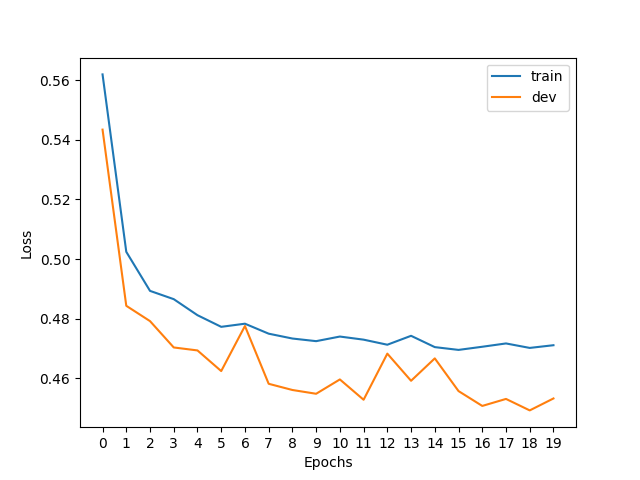
\includegraphics[width=0.7\textwidth]{hw1/single_run_loss.png}
\end{center}

Configuration: \texttt{glove-twitter-50}, batch size 64, Adam at learning rate 0.025, 20 epochs.
Selected values from the run:

\begin{center}
\begin{tabular}{|l|r|r|r|r|r|r|}
  \hline
  Epoch & 0 & 5 & 10 & 15 & 17 & 19 \\
  \hline
  Train loss & 0.5619 & 0.4772 & 0.4740 & 0.4695 & 0.4717 & 0.4711 \\
  Dev loss & 0.5434 & 0.4624 & 0.4596 & 0.4557 & 0.4531 & 0.4532 \\
  Dev acc & 0.7140 & 0.7930 & 0.7850 & 0.7880 & 0.7940 & 0.7950 \\
  \hline
\end{tabular}
\end{center}

Test set: loss 0.4679, accuracy 0.7950. Minimum dev loss 0.4492 at epoch 18.

\textbf{Findings.}
Train loss drops steeply for three epochs, then both curves flatten and the dev curve never turns
upward, so the model is not overfitting: $50 \times 2 + 2 = 102$ trainable parameters against 20,000
examples. Dev loss settles below train loss, near 0.452 against 0.471, and over the final ten epochs
its spread is four times as wide because it is measured on only 1,000 examples. The shared plateau is a
limit of the representation rather than the optimizer, because averaging 50-dimensional word vectors 
discards word order and negation.

\subsection*{5.2.8 Run the pipeline: Explore Different Word Embeddings}

\begin{center}
  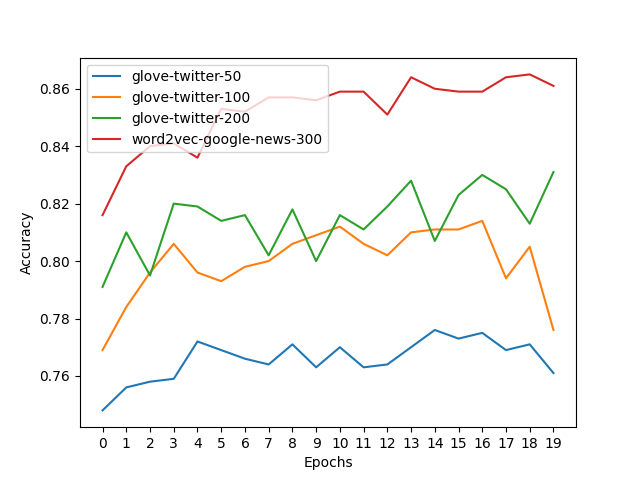
\includegraphics[width=0.625\textwidth]{hw1/embedding_acc.png}
\end{center}
\begin{center}
  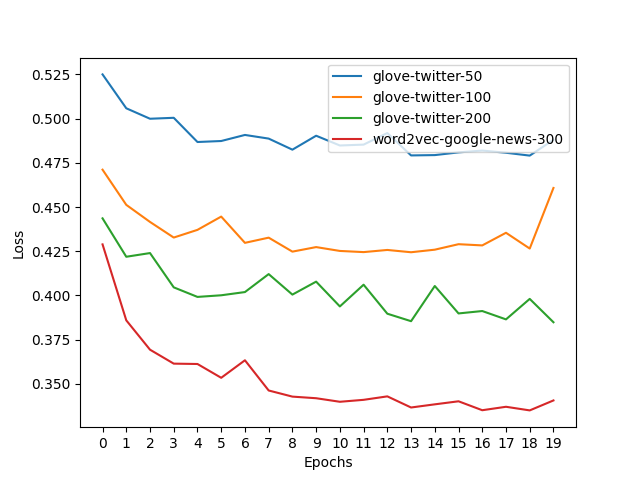
\includegraphics[width=0.625\textwidth]{hw1/embedding_loss.png}
\end{center}

Measured results across the four configurations, with vocabulary size and token coverage computed
over a 500-review sample of the test split (139,530 tokens):

\begin{center}
\small
\begin{tabular}{|l|r|r|r|r|r|r|}
  \hline
  Embedding & Dim & Params & Vocab & Token cov. & Final dev loss & Test acc. \\
  \hline
  \texttt{glove-twitter-50} & 50 & 102 & 1,193,514 & 97.8\% & 0.4880 & 0.772 \\
  \texttt{glove-twitter-100} & 100 & 202 & 1,193,514 & 97.8\% & 0.4608 & 0.803 \\
  \texttt{glove-twitter-200} & 200 & 402 & 1,193,514 & 97.8\% & 0.3848 & 0.821 \\
  \texttt{word2vec-google-news-300} & 300 & 602 & 3,000,000 & 74.5\% & 0.3406 & 0.846 \\
  \hline
\end{tabular}
\end{center}

\textbf{Findings.}
All three GloVe-Twitter runs share one vocabulary and identical 97.8\% token coverage, so width is the
only variable, and test accuracy climbs 0.772 to 0.803 to 0.821. Yet \texttt{word2vec-google-news-300}
wins at 0.846 with only 74.5\% token coverage, because it omits \texttt{a}, \texttt{of}, \texttt{and},
\texttt{to}, and all punctuation, which acts as a free stopword filter on the average. I would not credit
that to width alone, though, since it also changes training corpus and algorithm.

\end{document}
